%\documentclass[compress,t,11pt]{beamer}
\documentclass[handout,compress,t,11pt]{beamer}
\usetheme[]{metropolis}           % Use metropolis theme
\usefonttheme{serif}
\definecolor[named]{Gray}{RGB}{111,112,114}
\definecolor[named]{DarkGray}{RGB}{48,48,48}
\definecolor[named]{Cardinal}{RGB}{179,22,34}
\usepackage[T1]{fontenc}
\usepackage[altbullet]{lucidabr}
\usepackage{textcomp}
\usepackage{upquote} % needed to make straight quotes work in listings
\usepackage{listgolang}
\usepackage{mathtools}
\usepackage{comment}
\usepackage{tikz}
\usepackage{tikzsymbols}
 \usetikzlibrary{trees,shapes,plotmarks,arrows,er,automata,petri,topaths,positioning}
\usepackage{pifont}
\usepackage{clrscode}
\usepackage{setspace}
\usepackage{soul}
\usepackage{hyperref}
\usepackage{multirow}
\usepackage{array}

\setbeamercolor{palette primary}{fg=white,bg=Cardinal}
\setbeamercolor{palette secondary}{fg=white,bg=Gray}
\setbeamercolor{palette tertiary}{fg=white,bg=Cardinal}
\setbeamercolor{palette quaternary}{fg=white,bg=Gray}
\setbeamercolor{palette sidebar primary}{fg=white,bg=Cardinal}
\setbeamercolor{palette sidebar secondary}{fg=white,bg=Gray}
\setbeamercolor*{titlelike}{fg=Cardinal}
\setbeamercolor{structure}{fg=Gray}
\setbeamercolor{title separator}{fg=Cardinal}
\setbeamercolor{alerted text}{fg=Cardinal}
\setbeamercolor{reversed}{fg=Cardinal,bg=black}

\newcommand{\card}[1]{\ensuremath{\left|#1\right|}}
\newcommand{\norm}[1]{\ensuremath{\|#1\|}}

\title[Programming in Go]{\bf Programming in Go\\ Lesson 5: Concurrency}
\author{Matt Holiday} 
\institute[CP]{Cardinal Peak}
\date{14 May 2019} 
%\titlegraphic{\hfill
\includegraphics[width=.25\textwidth,height=.25\textheight]{cp-logo-2x.png}}
\titlegraphic{
\begin{tikzpicture}[overlay, remember picture,scale=0.4]
\node[at=(current page.north east), anchor=north east] (a) {};
\node[below left = 0.1cm and 0.1cm of a] (b)
{
\includegraphics[width=.25\textwidth,height=.25\textheight]{cp-logo-2x.png}};
\node[below left=2.56cm and 2.9cm of b]
{
\includegraphics[width=.1\textwidth]{go-logo.png}};
\end{tikzpicture}}

\setbeamerfont{footline}{series=\bfseries\selectfont}
\setbeamersize{text margin left=12pt,text margin right=12pt}
\linespread{1.0}
\metroset{block=fill}

\hypersetup{
    colorlinks=true,
    linkcolor=Cardinal,
    filecolor=magenta,      
    urlcolor=blue,
}

\begin{document}
\frame{\titlepage} 

%\section{Introduction}
\begin{frame}[fragile]
    \frametitle{Lesson \#5}
    What we'll cover today:
    \begin{itemize}
    \item Homework \#4
    \item Concurrent programming in Go
    \item Goroutines
    \item Channels
    \item Select
    \item Mutexes and package sync
    \end{itemize}
\end{frame}

% =================================================================================


\begin{frame}[fragile]
    \frametitle{Homework \#4}
\begin{golang}
package main

import (
	"fmt"
	"log"
	"net/http"
	"strconv"
)

// NOTE: don't do this in real life
type dollars float32

func (d dollars) String() string {
	return fmt.Sprintf("$%.2f", d)
}

type database map[string]dollars
\end{golang}
\end{frame}

\begin{frame}[fragile]
    \frametitle{Homework \#4}
\begin{golang}
func (db database) list(w http.ResponseWriter, 
                        req *http.Request) {
	for item, price := range db {
		fmt.Fprintf(w, "%s: %s\n", item, price)
	}
}

func (db database) add(w http.ResponseWriter, 
                       req *http.Request) {
	item := req.URL.Query().Get("item")
	price := req.URL.Query().Get("price")

	if _, ok := db[item]; ok {
		w.WriteHeader(http.StatusBadRequest) // 400

		fmt.Fprintf(w, "duplicate item: %q\n", item)
		return
	}
\end{golang}
\end{frame}

\begin{frame}[fragile]
    \frametitle{Homework \#4}
\begin{golang}
	if f64, err := strconv.ParseFloat(price, 32); err != nil {
		w.WriteHeader(http.StatusBadRequest) // 400

		fmt.Fprintf(w, "invalid price: %q\n", price)
	} else {
		db[item] = dollars(f64)

		fmt.Fprintf(w, "added %s with price %s\n", item, 
                    dollars(f64))
	}
}

func (db database) update(w http.ResponseWriter,
                          req *http.Request) {
	item := req.URL.Query().Get("item")
	price := req.URL.Query().Get("price")
\end{golang}
\end{frame}

\begin{frame}[fragile]
    \frametitle{Homework \#4}
\begin{golang}
	if _, ok := db[item]; !ok {
		w.WriteHeader(http.StatusNotFound) // 404

		fmt.Fprintf(w, "no such item: %q\n", item)
		return
	}

	if f64, err := strconv.ParseFloat(price, 32); err != nil {
		w.WriteHeader(http.StatusBadRequest) // 400

		fmt.Fprintf(w, "invalid price: %q\n", price)
	} else {
		db[item] = dollars(f64)

		fmt.Fprintf(w, "new price %s for %s\n", dollars(f64), 
                    item)
	}
}
\end{golang}
\end{frame}

\begin{frame}[fragile]
    \frametitle{Homework \#4}
\begin{golang}
func (db database) fetch(w http.ResponseWriter,
                         req *http.Request) {
	item := req.URL.Query().Get("item")

	if _, ok := db[item]; !ok {
		w.WriteHeader(http.StatusNotFound) // 404

		fmt.Fprintf(w, "no such item: %q\n", item)
		return
	}

	fmt.Fprintf(w, "item %s has price %s\n", item, 
                db[item])
}
\end{golang}
\end{frame}

\begin{frame}[fragile]
    \frametitle{Homework \#4}
\begin{golang}
func (db database) drop(w http.ResponseWriter,
                        req *http.Request) {
	item := req.URL.Query().Get("item")

	if _, ok := db[item]; !ok {
		w.WriteHeader(http.StatusNotFound) // 404

		fmt.Fprintf(w, "no such item: %q\n", item)
		return
	}

	delete(db, item)
	fmt.Fprintf(w, "dropped %s\n", item)
}
\end{golang}
\end{frame}

\begin{frame}[fragile]
    \frametitle{Homework \#4}
\begin{golang}
func main() {
	db := database{"shoes": 50, "socks": 5}

	http.HandleFunc("/list", db.list)
	http.HandleFunc("/create", db.add)
	http.HandleFunc("/update", db.update)
	http.HandleFunc("/delete", db.drop)
	http.HandleFunc("/read", db.fetch)

	log.Fatal(http.ListenAndServe("localhost:8000", nil))
}
\end{golang}
\end{frame}

% =================================================================================

\section{Share memory by communicating}
\begin{frame}[fragile]
    \frametitle{Concurrency}
    It's when you need to deal with two things at the same time \par
    \vspace{0.5\baselineskip}
   
    Parallelism expands that --- two things happen at the same time \par
    \vspace{2\baselineskip}
    You can have concurrency with a single-core processor \par
    \vspace{1.5\baselineskip}
    We need it to take advantage of multi-core processing: chips
    aren't getting faster as fast as they used to \par
    \vspace{2\baselineskip}
    It's not avoidable --- so how to deal with it?
\end{frame}

\begin{frame}[fragile]
    \frametitle{Communicating sequential processes}
    A model for thinking about concurrency that makes it {\em less} hard \par
    \vspace{\baselineskip}
    It's always hard: the human brain wasn't made to think this way \par
    \vspace{2\baselineskip}
    There's a lot of push now for event-driven or ``reactive'' models ---
    they're {\bf hard} hard \par
    \vspace{1.5\baselineskip}
    How about a simple program that talks to another program? \par
    \vspace{1.5\baselineskip}
    That's what CSP is about --- break your program into nanoservices
\end{frame}

\begin{frame}[fragile]
    \frametitle{Goroutines}
    A goroutine isn't a thread, but you can think of it that way \par
    \vspace{2\baselineskip}
    It's easy to start a goroutine \par
    \vspace{\baselineskip}
    The trick is knowing how the goroutine will stop: 
    \begin{itemize}
        \item you have a well-defined loop terminating condition
        \item you have a channel that closes to signal completion
        \item you let it run until the program stops
    \end{itemize}
    \vspace{1.5\baselineskip}
    But you need to make sure it doesn't get blocked by mistake 
\end{frame}

\begin{frame}[fragile]
    \frametitle{Channels}
    A channel is like a one-way socket or a Unix pipe \par
    \vspace{2\baselineskip}
    It's a method of synchronization as well as communication  \par
    \vspace{\baselineskip}
    We know that a write always {\em happens before} a read  \par
    \vspace{2\baselineskip}
    It's also a vehicle for transferring ownership of data, so that
    only one goroutine at a time is writing the data \par
    \vspace{\baselineskip}
    ``Don't communicate by sharing memory; instead, {\bf share memory by 
        communicating}.'' --- Rob Pike
\end{frame}

\begin{frame}[fragile]
\frametitle{Simple example}
\begin{golang}
results := make(chan int)

// asynchronously yield a stream of integers

go func(limit int, out chan<- int) {
    for i := 0; i < limit; i++ {
        out <- i
    }

    close(out)  // else we would deadlock
}(10, results)

// receive them when they're ready

for i := range results {
    fmt.Println(i)
}
\end{golang}
\end{frame}

\begin{frame}[fragile]
    \frametitle{Channels}
    A goroutine blocks waiting to read an empty channel \par
    \vspace{\baselineskip}
    A goroutine blocks waiting to write to a full channel  \par
    \vspace{2.5\baselineskip}
    Some channels have buffers, so that a writer doesn't wait  \par
    \vspace{3\baselineskip}
    We need to make sure goroutines don't block forever \par
    \vspace{\baselineskip}
    One way to do that is multiplexing with \verb|select|
\end{frame}

\begin{frame}[fragile]
    \frametitle{Select}
    \verb|select| allows any ``ready'' alternative to proceed among
    \begin{itemize}
        \item a channel we can read from
        \item a channel we can write to
        \item a \verb|default| action that's always ready
    \end{itemize}
    \vspace{\baselineskip}
    Most often \verb|select| runs in a loop so we keep trying  \par
    \vspace{2\baselineskip}
    We can put a timeout or ``done'' channel into the \verb|select|  \par
    \vspace{\baselineskip}
    That gives us a way out
\end{frame}

\begin{frame}[fragile]
    \frametitle{Select}
\begin{golang}
for {
	select {
	case x, ok := <- data:
        if !ok {
            break
        }

		// use the data ...

    case <-time.After(30 * time.Second):
        // safety timeout (one-shot channel)
        return
	}
}
\end{golang}
    \vspace{\baselineskip}
If we put a \verb|default| here, we'd busy wait
\end{frame}

\begin{frame}[fragile]
    \frametitle{Two ways to block a goroutine}
An empty \verb|select| blocks but consumes no CPU
\begin{golang}
for {}       // blocks by spinning

select {}    // blocks by sleeping
\end{golang}
\end{frame}

% =================================================================================

\section{Asynchronous Logging Example}
\begin{frame}[fragile]
    \frametitle{How channels solve problems}
Example thanks to Bill Kennedy's 
\href{https://www.youtube.com/watch?v=zDCKZn4-dck}{Behavior of Channels}\par
\vspace{2\baselineskip}
We'll build a program where the log device may have a problem \par
\vspace{2\baselineskip}
When this happens, we don't want the program to hang . . .
\end{frame}

\begin{frame}[fragile]
    \frametitle{Logger with an issue}
\begin{golang}
type device struct {
    problem bool
}

func (d *device) Write(p []byte) (int, error) {
    for d.problem {
        time.Sleep(time.Second)
    }

    return fmt.Println(string(p))
}

func main() {
    var d device
    var l log.Logger
    
    l.SetOutput(&d)
    . . . 

\end{golang}
\end{frame}

\begin{frame}[fragile]
    \frametitle{Logger with an issue}
\begin{golang}
    . . .
    for i := 0; i < 10; i++ {
        go func(id int) {
            for {
                l.Println(fmt.Sprintf("%d: log data", id))
                time.Sleep(100 * time.Millisecond)
            }
        }(i)
    }

    sigChan := make(chan os.Signal, 1)
    signal.Notify(sigChan, os.Interrupt)

    for {
        <- sigChan
        d.problem = !d.problem
    }
}
\end{golang}
\end{frame}

\begin{frame}[fragile]
    \frametitle{Custom logger}
\begin{golang}
type Logger struct {
    ch chan string
    wg sync.WaitGroup
}

func (l *Logger) Stop() {
    close(l.ch)
    l.wg.Wait()
}

func (l *Logger) Println(s string) {
    select {
    l.ch <- s + "\n":
        // do nothing
    default:
        fmt.Println("DROP")
    }
}
\end{golang}
\end{frame}

\begin{frame}[fragile]
    \frametitle{Custom logger}
\begin{golang}
func New(w io.Writer, cap int) *Logger {
    l := Logger{
        ch: make(chan string, cap)
    }
    
    l.wg.Add(1)

    go func() {
        for v := range l.ch {
            fmt.Fprintf(w, v)
        }

        l.wg.Done()
    }()

    return &l
}
\end{golang}
\end{frame}

\begin{frame}[fragile]
    \frametitle{Custom logger}
\begin{golang}
func main() {
    d := device{}
    l := New(&d, 10)

    // same code as before; spin off 10 goroutines
    // and accept ctrl-C to create a problem
    . . .
}
\end{golang}
\vspace{2\baselineskip}
If we hit \verb|Ctrl-C| now, the buffer fills and we drop logs ... \par
\vspace{2\baselineskip}
Buffered channels and a \verb|select| allowed us to avoid deadlock
\end{frame}


% =================================================================================

\section{Audio Forwarding Example}

\begin{frame}[fragile]
    \frametitle{Audio forwarding}
    In this example, we read audio from a websocket and forward it
    to an HTTP connection \par
    \vspace{\baselineskip}
    We need to stop forwarding once we've received the correct
    indication back from the web server, or detected end-of-speech \par
    \vspace{\baselineskip}
    We need a new goroutine, a couple of channels, and a \verb|select|
    \vspace{\baselineskip}
\begin{center}
    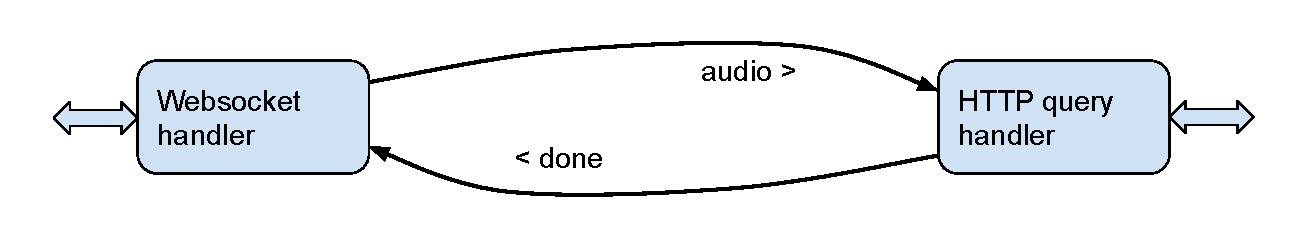
\includegraphics[width=\textwidth]{audio-forward.pdf}
\end{center}
\end{frame}


\begin{frame}[fragile]
    \frametitle{Audio forwarding}
\begin{golang}
func (h *houndASR) AddAudio(audio []byte) error {
	if h.eos { return types.ErrEndOfSpeech }
	if h.done == nil { // start up on first chunk
		h.done = make(chan bool, 1)
		h.input = make(chan []byte, 32)
		go h.runQuery(&sender{ch: h.input})
	}

	h.input <- audio

	select {
	case done, ok := <-h.done:
		if !ok || done { h.eos = true }
	default:
		if h.tracker.DetectedEOS(audio) { h.eos = true }
	}

	if h.eos { close(h.input) }; return nil
}
\end{golang}
\end{frame}

\begin{frame}[fragile]
    \frametitle{Audio forwarding}
\begin{golang}
func (h *houndASR) runQuery(sdr *sender) {
	req, _ := http.NewRequest("POST", h.voiceURL, sdr)
    resp, _ := h.client.Do(req)
	reader := bufio.NewReader(resp.Body)
	defer resp.Body.Close()

	for {
		bytes, _ := reader.ReadBytes('\n') // chunked resp
		data := transcript{}

		if err := json.Unmarshal(bytes), &data); err != nil {
            break
        }
        if data.Done {
		    h.done <- true
        }
        . . .
    }
}
\end{golang}
\end{frame}


\begin{frame}[fragile]
    \frametitle{Audio forwarding}
\begin{golang}
type sender struct {
	ch chan []byte
}

func (s *sender) Read(p []byte) (n int, err error) {
	v, ok := <-s.ch  // blocking read

	if !ok {
		return 0, io.EOF
	}

	// assume for now it fits
	return copy(p, v), nil
}

func (s *sender) Close() error {
	return nil
}
\end{golang}
\end{frame}

% =================================================================================

\section{Conventional Synchronization}

\begin{frame}[fragile]
    \frametitle{Conventional synchronization}
    Package \verb|sync| with \verb|Mutex|, \verb|WaitGroup|, etc. \par
    \vspace{\baselineskip}
    Package \verb|sync/atomic| for atomic scalar reads \& writes \par
    \vspace{2\baselineskip}
    We saw a use of wait groups in the 2nd example above  \par
    \vspace{2\baselineskip}
    Mutexes must be locked \& unlocked to give protection \par
    \vspace{\baselineskip}
    Mutexes block a goroutine when locked by another
\end{frame}

\begin{frame}[fragile]
    \frametitle{Mutexes in action}
\begin{golang}
type safeMap struct {
    sync.Mutex         // not safe to copy
    m map[string]int
}

// so methods must take a pointer, not a value
func (s *safeMap) incr(key string) {
    s.Lock()
    defer s.Unlock()
    
    // only one goroutine can execute this
    // code at the same time, guaranteed
    s.m[key]++
}
\end{golang}
\vspace{\baselineskip}
Using \verb|defer| is a good habit, avoids mistakes
\end{frame}

\begin{frame}[fragile]
    \frametitle{Atomic primitives}
\begin{golang}
import "sync"

func do() int {
    var n int64
    var w sync.WaitGroup

    for i := 0; i < 1000; i++ {
        w.Add(1)

        go func() {
			n++                         // DATA RACE
            w.Done()
        }()
    }
    
    w.Wait()
    return n
}
\end{golang}
\end{frame}

\begin{frame}[fragile]
    \frametitle{Atomic primitives}
\begin{golang}
import ( "sync"; "sync/atomic" )

func do() int {
    var n int64
    var w sync.WaitGroup

    for i := 0; i < 1000; i++ {
        w.Add(1)

        go func() {
			atomic.AddInt64(&n, 1)      // fixed
            w.Done()
        }()
    }
    
    w.Wait()
    return n
}
\end{golang}
\end{frame}

% =================================================================================

\section{Some Gotchas}
\begin{frame}[fragile]
    \frametitle{Concurrency problems}
    \#1: race conditions, where unprotected writes overlap \par
    \begin{itemize}
        \item must be some data that is written to
        \item could be a read-modify-write operation
        \item and two goroutines can do it at the same time
    \end{itemize}
    \vspace{\baselineskip}
    \#2: deadlock, when no goroutine can make progress \par
    \begin{itemize}
        \item goroutines could all be blocked on empty channels
        \item goroutines could all be blocked waiting on a mutex
        \item GC could be prevented from running (busy loop)
    \end{itemize}
\vspace{\baselineskip}
Go detects most deadlocks; with \verb|-race| it can find data races
\end{frame}

\begin{frame}[fragile]
    \frametitle{Concurrency problems}
    \#3: goroutine leak
    \begin{itemize}
        \item goroutine hangs on a empty or blocked channel
        \item not deadlock: other goroutines make progress
        \item often found by looking at pprof output
    \end{itemize}
    \vspace{0.6\baselineskip}
    When you start a goroutine, \alert{\bf always know how/when it will end} \par
    \vspace{1.4\baselineskip}
    \#4: other errors
    \begin{itemize}
        \item misuse of \verb|Mutex|
        \item misuse of \verb|WaitGroup|
        \item misuse of \verb|select|
    \end{itemize}
\end{frame}

\begin{frame}
    \frametitle{Gotchas 1: Deadlock}
    A goroutine is {\bf preemptible} only when it starts a (non-inlined)
    function call, blocks on a channel or mutex, or makes a blocking system call
    \vspace{\baselineskip}
\begin{alertblock}{Potential Problems}
    If your goroutine isn't preemptible, garbage collection will never run,
    because it must first ``stop the world''
\end{alertblock}
    \vspace{\baselineskip}
    However, if the {\tt main()} function exits, all goroutines terminate
\end{frame}

\begin{frame}[fragile]
    \frametitle{Gotchas 1: Deadlock example}
\begin{golang}
go func() {
    var i byte

    for i = 0; i <= 255; i++ {
        // infinite loop does nothing
        // doesn't get elided
        // and can't be preempted
    }
}()

runtime.Gosched()    // yield execution
runtime.GC()         // force GC

// DEADLOCK

fmt.Println("Done")  // never happens
\end{golang}
\end{frame}

\begin{frame}[fragile]
    \frametitle{Gotchas 1: Deadlock fixed}
\begin{golang}
go func() {
    var i byte

    for i = 0; i <= 255; i++ {
        // infinite loop does nothing
        // doesn't get elided

        // but we can yield
		if (i == 123) {
			runtime.Gosched()
		}
    }
}()

runtime.Gosched()    // yield execution
runtime.GC()         // force GC
fmt.Println("Done")  // prints Done
\end{golang}
\end{frame}

\begin{frame}[fragile]
    \frametitle{Gotchas 2: Closure capture}
    A closure shouldn't capture a {\bf mutating} variable, e.g. a loop index \par
    \vspace{0.6\baselineskip}
    If it does, it will get the wrong value! \par
    \vspace{0.2\baselineskip}
\begin{golang}
for i := 0; i < 10; i++ {   // WRONG
    go func() {
        fmt.Println(i)
    }()
}
\end{golang}
    Instead, \alert{\bf pass the variable's value as a parameter}
    \vspace{0.2\baselineskip}
\begin{golang}
for i := 0; i < 10; i++ {  // RIGHT
    go func(i int) {
        fmt.Println(i)
    }(i)
}
\end{golang}
\end{frame}

\begin{frame}[fragile]
    \frametitle{Gotchas 3: Goroutine leak}
    In this example, a timeout leaves the goroutine hanging forever \par
\begin{golang}
func finishReq(timeout time.Duration) *obj {
    ch := make(chan obj)

    go func() {
        ch <- fn() // blocking send
    }()

    select {
    case rslt := <-ch:
        return rslt
    case <-time.After(timeout):
        return nil
    }
}
\end{golang}
    \vspace{0.2\baselineskip}
    The correct solution is to make a buffered channel
\end{frame}

\begin{frame}[fragile]
    \frametitle{Gotchas 4: Incorrect use of WaitGroup}
    Always, always, always call \verb|Add| before \verb|go| or \verb|Wait| \par
    \vspace{0.4\baselineskip}
\begin{golang}
func walkDir(dir string, pairs chan<- pair, ...) {
    wg.Add(1)                                      // WRONG
	defer wg.Done()

	visit := func(p string, fi os.FileInfo, ...) {  
		if fi.Mode().IsDir() && p != dir {
			go walkDir(p, pairs, wg, limits)
        . . .
}

err := walkDir(dir, paths, wg)
wg.Wait()
\end{golang}
    \vspace{\baselineskip}
    Adding too late may cause \verb|Wait| to return too soon
\end{frame}

\begin{frame}[fragile]
    \frametitle{Gotchas 4: Incorrect use of WaitGroup}
    Adding inside \verb|walkDir| (and not before) may have
    a timing problem
\begin{center}
    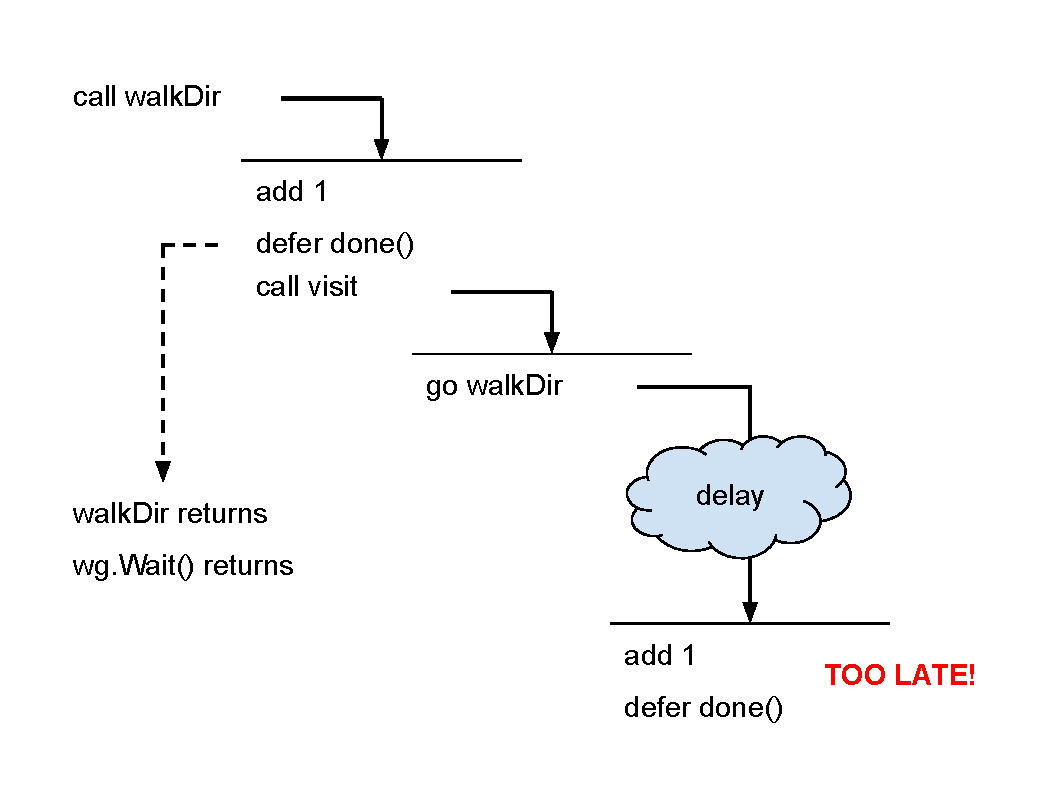
\includegraphics[height=.75\textheight]{waitgroup-error.pdf}
\end{center}
\end{frame}

\begin{frame}[fragile]
    \frametitle{Gotchas 4: Incorrect use of WaitGroup}
    Always, always, always call \verb|Add| before \verb|go| or \verb|Wait| \par
    \vspace{0.4\baselineskip}
\begin{golang}
func walkDir(dir string, pairs chan<- pair, ...) {
	defer wg.Done()

	visit := func(p string, fi os.FileInfo, ...) {  
		if fi.Mode().IsDir() && p != dir {
            wg.Add(1)                              // RIGHT
			go walkDir(p, pairs, wg, limits)
        . . .
}

wg.Add(1)                                          // RIGHT
err := walkDir(dir, paths, wg)
wg.Wait()
\end{golang}
    \vspace{0.4\baselineskip}
    Adding too late may cause \verb|Wait| to return too soon
\end{frame}

\begin{frame}[fragile]
    \frametitle{Some bad code for your delectation}
\begin{golang}
func do() {
    var wg sync.WaitGroup
    sem := make(chan int, 4)  // 4 simultaneous workers

    for i := 0; i < 10; i++ {
        wg.Add(1); sem <- 1

        go func() {
            defer func() {
                wg.Done(); <- sem
            }()
            
            // some work
        }()
    }

    wg.Wait(); close(sem)
}
\end{golang}
\end{frame}

\begin{frame}[fragile]
    \frametitle{Some bad code for your delectation}
    \begin{enumerate}
        \item the order of \verb|wg.Done| and \verb|<-sem| is confusing
        \vspace{0.6\baselineskip}
        \item read from a closed channel is safe, but \verb|close| isn't needed
        \vspace{0.6\baselineskip}
        \item we acquire the semaphore too soon, limiting the number of
              goroutines (not the number of simultaneous workers)
\begin{golang}
    for i := 0; i < 10; i++ {
        wg.Add(1)

        go func() {
            defer wg.Done()

            sem <- 1
            // some work
            <- sem
        }()
    }
\end{golang}
    \end{enumerate}    
\end{frame}

\begin{frame}[fragile]
    \frametitle{Select problems}
    \verb|select| can be challenging and lead to mistakes:
    \begin{itemize}
        \item \verb|default| is always active
        \vspace{0.3\baselineskip}
        \item a \verb|nil| channel is always ignored
        \vspace{0.3\baselineskip}
        \item a full channel (for send) is skipped over
        \vspace{0.3\baselineskip}
        \item available channels are selected at random
        \vspace{0.3\baselineskip}
        \item the ``done'' channel is just another channel
    \end{itemize}
    % \vspace{2\baselineskip}
    % Mistake \#1: skipping a full channel to default and losing a message  \par
    % \vspace{\baselineskip}
    % Mistake \#2: reading a ``done'' channel and aborting when input is backed
    % up on another channel --- that input is lost \par
\end{frame}

\begin{frame}[fragile]
    \frametitle{Anatomy of a select mistake: \#1}
    Mistake \#1: skipping a full channel to default and losing a message  \par
\begin{golang}
for {
    x := socket.Read()

    select {
    case output <- x:
        . . .
    
    default:
        return
    }
}
\end{golang}
The code was written assuming we'd skip \verb|output| only if it was set to 
\verb|nil| (as no longer needed) \par
\vspace{0.4\baselineskip}
We also skip if \verb|output| is full, and lose this and future messages
\end{frame}

\begin{frame}[fragile]
    \frametitle{Anatomy of a select mistake: \#2}
    Mistake \#2: reading a ``done'' channel and aborting when input is backed 
    up on another channel --- that input is lost \par
\begin{golang}
for {
    select {
    case x := <- input:
        . . .

    case <- done:
        return
    }
}
\end{golang}
    \vspace{0.6\baselineskip}
There's no guarantee we read all of \verb|input| before reading \verb|done| \par
    \vspace{0.6\baselineskip}
Better: use \verb|done| only for an error abort; close \verb|input| on EOF
\end{frame}

\begin{frame}[fragile]
    \frametitle{Some thoughts}
    Three considerations when using concurrency:
    \begin{enumerate}
    \item Don't start a goroutine without knowing how it will stop \par
        \vspace{0.6\baselineskip}
    \item Acquire locks/semaphores as late as possible; release them in
          the reverse order as soon as possible (and without fail)
        \vspace{0.6\baselineskip}
    \item Don't wait for non-parallel work that you could do yourself 
\begin{golang}
func do() int {
    ch := make(chan int)

    go func() { ch <- 1 }()

    return <-ch
}
\end{golang}
        \vspace{0.6\baselineskip}
    \item {\bf Simplify!} Make everything clear and easy to read!
    \end{enumerate}
\end{frame}

\begin{frame}[fragile]
\frametitle{Channel state reference}
{\renewcommand{\arraystretch}{1.5}
\begin{table}[h!]
  \begin{center}
    \begin{tabular}{l||l|l|l}%{m{2.5cm}||m{1.6cm}|m{1.6cm}|m{3.5cm}}
      \textbf{State} & \textbf{Receive}  & \textbf{Send} & \textbf{Close}\\
      \hline\hline
      Nil & Block* & Block* & Panic \\
      \hline
      Empty & Block & Write & Close \\
      \hline
      Partly Full & Read & Write & \multirow{2}{*}{Readable until empty} \\
      \cline{1-3}
      Full & Read & Block \\
      \hline
      Closed & Default Value** & \multicolumn{2}{c}{Panic} \\
      \hline\hline
      Receive-only & OK & \multicolumn{2}{c}{Compile Error} \\
      \hline
      Send-only & Compile Error & \multicolumn{2}{c}{OK} \\
    \end{tabular}
  \end{center}
\end{table}
}
{\footnotesize
  * \verb|select| ignores a nil channel since it would always block \\
  ** Reading a closed channel returns \verb|(<default-value>, !ok)|
}
\end{frame}


    % one goroutine reads from a socket, on error it closes
    % a done channel, otherwise data is pushed onto an input
    % channel that has a buffer
    %
    % the other goroutine reads from the input channel as
    % well as the cancellation channel
    %
    % in a select, we have no assurance of order; with a few
    % items in the buffered input channel, the done channel
    % may be selected, cause the 2nd goroutine to return and
    % so lose some of the buffered input!
    %
    % a better design is to close the input channel on error
    % and have the 2nd goroutine depend (as much as possible)
    % on the input channel closing; using the done channel
    % only to abort in a way were losing data is acceptable


    % we had a select which tried to push to a channel which
    % might be nilled out when no longer needed, and so
    % there was a default case to bail out
    %
    % unfortunately, that also meant that if the channel was
    % active but full, the default case would be taken and
    % messages might be lost ...

%============================================================================

% what's the meaning of CSP? we don't have callbacks, events, complex state machines
% instead, we have "normal" code that communicates with other pieces of code
% if programs make microservices, then CSP makes parts of programs into nanoservices
% and we can understand those parts a lot more easily (not that it's ever simple)
%
% goroutines - lightweight, cooperative; reduce the cost of context switching
% channels provide a powerful mechanism for communication; we can pass them around
% we can compose them to make sophisticated models we can still reason about

% a goroutine is an execution context; easy to think about it like a thread
% it can be a named function call, or the call of an anonymous function
%
% when we start one, we need to understand how it will end and make that happen
% if it's looping, when does that loop end?
% we don't want hung goroutines, as they waste lots of space (the garbage in GC)
%
% we can make goroutines end by
% a) making the loop range over something finite
% b) making a special "done" or "close" channel to signal that they should end
% c) letting them end when the program stops, because they're lifelong utilities
%
% goroutines get blocked: writing to a channel that's never read, or a nil channel
% or by reading a channel that gets no input / is not closed
%
% we need to make sure channels get closed when "all" the data has been pushed
%
% we need to understand that dumb logic bugs can cause goroutines to get stuck
% or get stuck in an endless loop
%
% part of the power of using channels is understanding them as vehicles to transfer
% ownership; and thus also see goroutines as objects that own things
%
% map-reduce: we have a collector which puts data into the final result and owns
% that data -- so there's no race condition updating it; and when done, the result
% gets transfered elsewhere through another channel
%
% if only one goroutine "owns" the object at any one time, then it's thread safe
%
% if that's not convenient, then use a traditional mutex / atomic op to protect it
%
% that's the point of "share memory by communicatng"
%

% =================================================================================

\section{Homework}

\begin{frame}[fragile]
\frametitle{Homework \#5}
{\small \setstretch{1.1}Take the program you wrote for Homework \#4, and write
another program using goroutines that drives it with multiple readers \& writers 
until it breaks due to the race conditions that were left unsolved. \par
    \vspace{0.4\baselineskip}
You will want to run the server with Go's \verb|-race| option to identify the 
failures. You may wish to write your driver program in the form of a \\
unit test. More info on the
\href{https://golang.org/doc/articles/race_detector.html}{race detector} is
on the Go site. \par
    \vspace{0.4\baselineskip}
(Re-use your HTTP read logic from Homework \#3. Feel free to extend your server \&
client to use JSON instead of URL parameters if you need more challenge.) \par
    \vspace{0.4\baselineskip}
Then add mutexes to the database so that it is protected against race conditions
and no longer fails with concurrent updates.}
\end{frame}

\end{document}
